\chapter{Entfaltung}
Vorerst wird das zugrundeliegende Problem in \autoref{sec:inverse_problem} aufgeführt und die Entfaltung diskutiert.
Im Anschluss wird in \autoref{sec:dsea} auf den Lösungsansatz mit DSEA eingegangen und der Algorithmus erläutert.
Das letzte Kapitel \autoref{sec:NN} befasst sich mit neuronalen Netzen und wie sie als Klassifikationsalgorithmus verwendet werden können.

% INVERSE PROBLEME
\section{Inverse Probleme} \label{sec:inverse_problem}
Inverse Probleme treten in der Physik überall da auf, wo die gesuchte physikalische Größe nicht \textit{direkt} messbar ist.
Die Neutrinoenergie ist nur \textit{indirekt} messbar.
Ziel ist die Rekonstruktion der gesuchten Größe, also der Neutrinoenergie aus der Messgröße.
In IceCube wird das Cherenkov-Licht der Zerfallsprodukte gemessen, siehe dazu \autoref{sec:icecube}.
\\
Mathematisch ist das Problem über die Fredholm-Integralgleichung\cite{twomey1963numerical} 
\begin{equation}
    \int_{\Omega} A(x,y) f(x) \mathrm{d}x + b(y) = g(y)
\end{equation}
definiert.
Die Verteilung des wahren Parameters $x$ wird durch $f(x)$ und die Verteilung der Messdaten durch $g(x)$ dargestellt.
Der gesamte Messprozess und die ablaufenden physikalischen Prozesse werden durch die Antwortfunktion $A(x,y)$ beschrieben.
Üblicherweise wird der Messprozess durch einen Untergrund $b(y)$ beeinflusst.
Dieser ist nicht von Interesse und kann mit Signal-Untergrund-Trennverfahren separiert werden.
\\
Im diskreten Fall werden die kontinuierlichen Verteilungen $f(x), g(y)$ zu \textbf{Vektoren} und $A(x,y)$ zu einer Antwort\textbf{matrix}.
Ohne Untergrund vereinfacht sich die Gleichung zu
\begin{equation}
    g_i = \sum_{j=1}^{n} A_{ij} f_j \, .
\end{equation}

Die Rekonstruktion der Größe $f$ wird als Entfaltung bezeichnet.
Der naive Ansatz über Bildung der Inverse von $A$ führt häufig zu unbrauchbaren Lösungen.
Kleine anfängliche Störungen verstärken sich und man erhält eine stark oszillierende Lösung.
Das Problem ist schlecht konditioniert und benötigt spezielle Ansätze.

% DSEA
\section{Lösungen mit DSEA} \label{sec:dsea}
Der \textbf{D}ortmund \textbf{S}pectrum \textbf{E}stimation \textbf{A}lgorithm (DSEA)\cite{ruhe,RockSolid2018DSEARR,boerner} betrachtet die Entfaltung als Klassifikationsproblem.
Vorab wird die Zielvariable $f(x)$ in $n$ Intervalle unterteilt:
\begin{equation}
    f(x) \rightarrow \vec{f}: \qquad f_j = \int_{y_{j-1}}^{y_j} f(x) \, \mathrm{d}x, \qquad j \in [1,n]
    \label{eq:diskretisierung}
\end{equation}
Jedes Intervall bzw. jeder Bin repräsentiert den in \autoref{eq:diskretisierung} definierten Energiebereich.
Die Bins stellen in DSEA die Zielklassen für eine Klassifikation dar.
\\
\\
DSEA ist ein iteratives Verfahren.
Im ersten Schritt wird ein Klassifikationsalgorithmus auf dem Datensatz ($X,W,F$) trainiert.
Dabei steht $X$ für die Features, die mit den Probengewichten $W$ gewichtet werden und $F$ für das Label.
DSEA geht von Daten mit gleichverteilten Klassen aus, d.h. die Gewichte $W$ werden dementsprechend initialisiert.
Dies hat den Vorteil, dass kein Prior angenommen werden muss und somit das Modell unabhängig von der Klassenverteilung im Trainingsdatensatz ist.
\\
Voraussetzung an den Klassifizier ist, dass dieser eine Konfidenz $c_{ij}$ ausgibt, die die Zugehörigkeit des $i$-ten Events zum $j$-ten Bin beschreibt.
Die Konfidenz wird als Wahrscheinlichkeit interpretiert.
\\
\\
Anschließend wird im 2. Schritt mit dem trainierten Klassifizierer/Modell eine Vorhersage für die zu entfaltenden Daten getroffen.
Über die für jedes Event $i$ und Bin $j$ erhaltende Konfidenz wird das Spektrum
\begin{equation}
    \hat{f}_{j} = \sum_{i=1}^{n} c_{ij}
    \label{eq:dsea_confidence}
\end{equation}
rekonstruiert, wobei $n$ die Anzahl der Datenpunkte angibt.
Die Konfidenzen werden für jeden Bin $j$ über alle Events aufsummiert und man erhält eine Vorhersage für den $j$-ten Bin des zu entfaltenden Spektrums $\hat{f}_j$.
\\
Im letzen (3.) Schritt werden die Probengewichte $w_{i}$
\begin{equation}
    w_{i} = \frac{f_{l_i}}{n}
\end{equation}
über das rekonstruierte Spektrum aktualisiert, wobei $l_i$ dem wahren Label des $i$-ten Events entspricht.
Die Gewichte entsprechen dem normierten Spektrum.
\\
Die erste DSEA-Iteration ist hiermit vollendet.
Anschließend wird wieder Schritt 1 ausgeführt und der Klassifizier mit angepassten Probengewichten trainiert.
Es werden soviele Iterationen ausgeführt bis Konvergenz eintritt.


% NEURONALE NETZE
\section{Neuronale Netze als Klassifikationsalgorithmus} \label{sec:NN}
Grundsätzlich kann jeder Klassifizierer verwendet werden, der für jede Zielklasse eine Konfidenz $c_{ij}$ ausgibt.
Beliebte Klassifikationsalgorithmen in DSEA sind Naive Bayes oder auch der Random Forest.
In dieser Arbeit werden neuronale Netze (\textbf{NN}) als Klassifizier in DSEA untersucht.
\begin{figure}
    \centering
    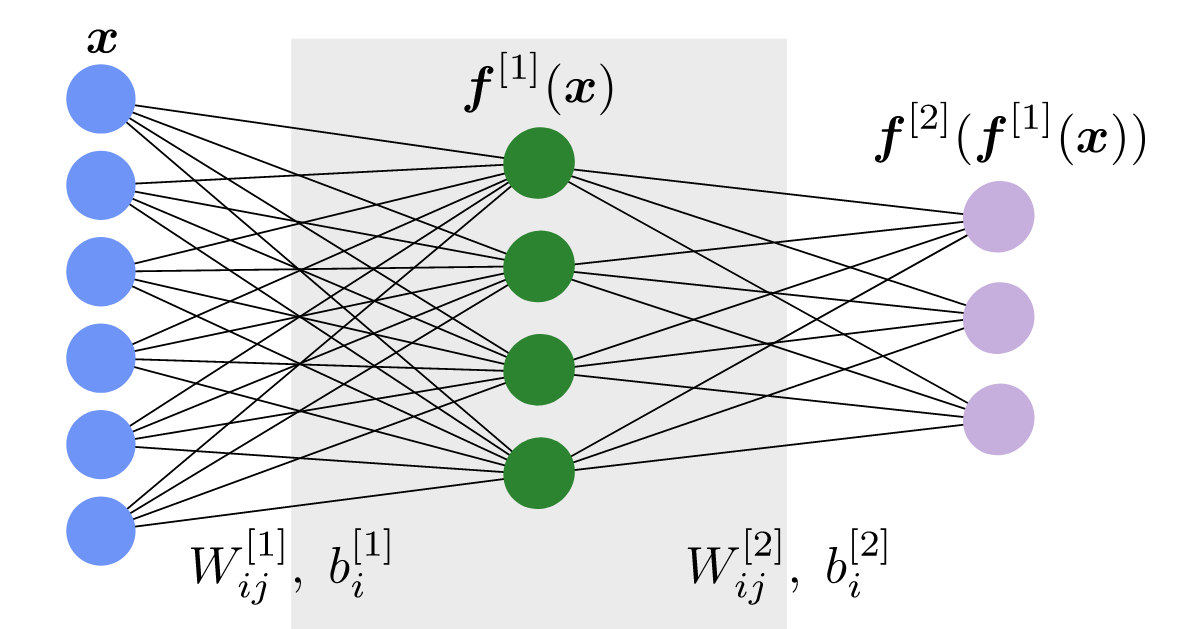
\includegraphics[width=0.8\textwidth]{Plots/nn_structure.png}
    \caption[Struktur eines NN mit einer tiefen Ebene]{Darstellung der Struktur eines einfachen neuronalen Netzes.
    Die blauen Kreise stellen die Neuronen der Eingansebene, die Grünen der tiefen Ebene und die Blauen der Ausgangsebene dar.
    Jedes Neuron besitzt zwei Parameter, eine Gewichtsmatrix $\mathbf{W}_{ij}$ und einen Biasvektor $\vec{b}_i$.
    Das Resultat für jede Ebene wird durch $f(x)$ beschrieben \cite{Neupert2021IntroductionTM}.
    }
    \label{fig:nn_structure}
\end{figure}
Das NN in \autoref{fig:nn_structure} beinhaltet drei Ebenen, wobei jede Ebene eine bestimmte Anzahl an Neurononen enthält.
Die Eingangsebene (Blau) besteht aus so vielen Neuronen, wie Features verwendet werden.
Jedes Neuron erhält also als Eingang ein Feature.
Es können beliebig viele tiefe Ebenen (Grün) verwendet werden.
Die Verbindungen zwischen zwei Ebenen wird durch die Gewichtsmatrix $\mathbf{W}$, den Biasvektor $\vec{b}$ und einer Aktivierungsfunktion $g(\vec{x})$ nach
\begin{equation*}
    g(f(\vec{x})) = g(\mathbf{W} \vec{x} + \vec{b})
\end{equation*}
beschrieben, wobei $\vec{x}$ den Ausgang aus der vorherigen Ebene beschreibt.
Es gibt eine große Auswahl an Aktivierungsfunktionen\cite{activationf}.
\begin{figure}
    \centering
    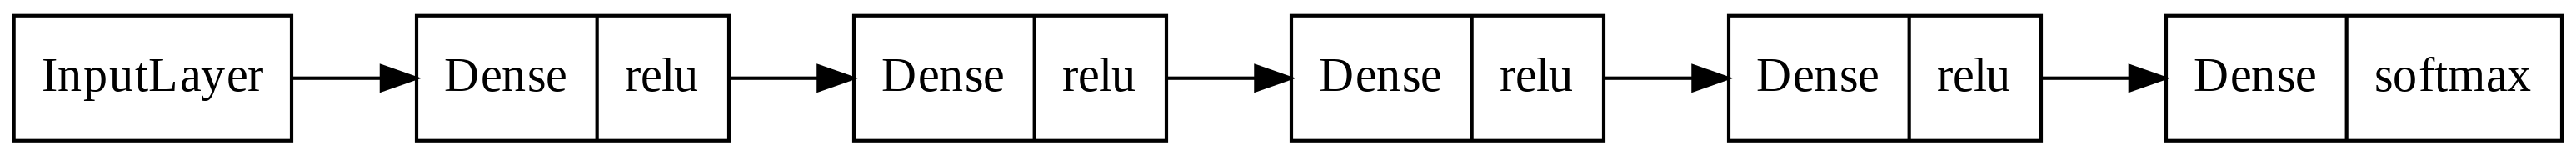
\includegraphics[width=\textwidth]{Plots/model_structure.png}
    \caption[Aufbau des verwendeten NN]{Der Aufbau des NN schematisch dargestellt.
    Nach der Eingangsebene folgen mehrere tiefe Ebenen mit der Aktivierungsfunktion ReLU.
    Die Verbindungen der letzten Ebene werden durch die Softmax-Funktion definiert.
    \label{fig:nn_aufbau}
    }
\end{figure}
Große NN mit vielen Parametern haben den Nachteil sich stark an die Daten anzupassen (Bias).
Bei dem in dieser Arbeit verwendeten NN handelt es sich um ein tiefes neuronales Netz mit etwa $\SI{60000}{\text{Parametern}}$.
Die Struktur ist in \autoref{fig:nn_aufbau} graphisch dargestellt.
Für quantitative Angaben der Ein- und Ausgangsdimensionen siehe \autoref{tab:nn_shape}.
Der einfache Aufbau soll zu einem geringen Bias im Modell führen.
\\
In den tiefen Ebenen wird die Aktivierungsfunktion \textit{ReLU} (\textbf{Re}ctified \textbf{L}inear \textbf{U}nit)
\begin{equation*}
    g_\text{ReLU}(x)=
        \begin{cases}
            x & {\text{if }} x \geq 0,\\
            0 & {\text{otherwise}}
        \end{cases}
\end{equation*}
genutzt.
Ist der Eingang $x$ größer 0, so wird dieser unverändert weitergegeben, sonst 0.
\\
Die Ausgangsebene enthält genauso viele Neuronen, wie es Zielklassen gibt.
In dieser Ebene wird die Aktivierungsfunktion Softmax verwendet.
Wie die Definition
\begin{equation*}
    g_\text{Softmax}(x_i) = \frac{\exp(x_i)}{\sum_j \exp(x_j)} \, .
\end{equation*}
zeigt, ist die Summe über alle Klassen für jedes Event gleich eins.
Sie erfüllt damit die Vorgabe an DSEA, dass für jede Zielklasse eine Konfidenz $c_{ij}$ ausgegeben wird.
\\
Die Kostenfunktion \textit{kategorische Kreuzentropie}\cite{cross_entropy} kann für ein Klassifikationsproblem verwendet werden.
Ziel ist die Minimierung der Kosten in Abhängigkeit der Modellparameter.
Die Minimierung der Kreuzentropie ist äquivalent zu einer Maximierung der Log-Likelihood-Funktion.
\\
Mit dem Optimierer \textit{ADAM} (Adaptive Moment Estimation)\cite{ADAM} wird die Kostenfunktion minimiert.
Der Algorithmus ist eine Erweiterung des Gradientenverfahrens und beachtet zusätzlich zu der Steigung das Moment.
Bildlich gesehen entspricht dies einer Kugel, die in einer hügeligen Landschaft Richtung globalem Minimum rollt und dabei lokale Minima überwindet.
Die Lernrate stellt ein Hyperparameter des Optimierers dar und ist ein Maß für die Schrittweite entlang des fallenden Gradienten.
\\
Das Modell wird auf einem Teil der Daten trainiert und evaluiert.
Dazu wird der Datensatz in mehrere Unter-Datensätze mit einer spezifizierten Größe (\textit{Batch Size})\cite{brownlee2018difference} unterteilt.
Das Modell wird auf einem Batch trainiert und die Kostenfunktion ausgewertet.
Wird dies für alle Batches durchgeführt, so wurde jeder Datenpunkt im Training einmal berücksichtigt.
Durch das häufige Anpassen der Parameter konvergiert die Kostenfunktion schneller.
\\
Das Modell wird mehrfach auf den Trainingsdaten trainiert.
Die Anzahl der Trainingsprozesse wird durch die \textit{Epochenzahl}\cite{brownlee2018difference} angegeben.